\documentclass[a4,useAMS,usenatbib,usegraphicx]{latex/mn2e} 
%\documentclass{latex/emulateapj} 
%External Packages and personalized macros
%=========================================================================
%		EXTERNAL PACKAGES
%=========================================================================
\usepackage{amsmath} 
\usepackage{amssymb} 
\usepackage[section]{placeins}
\usepackage {graphicx}
%\usepackage{graphics}
\usepackage[dvips]{epsfig}
\usepackage{epsfig}  
\usepackage{color}
\usepackage[normalem]{ulem}
\usepackage{hyperref}
\usepackage{caption}
%Non reposionated tables
\usepackage{float}
\restylefloat{table}

%=========================================================================
%		INTERNAL MACROS
%=========================================================================
\def\be{\begin{equation}}
\def\ee{\end{equation}}
\def\ba{\begin{eqnarray}}
\def\ea{\end{eqnarray}}

% To highlight comments 
\definecolor{red}{rgb}{1,0.0,0.0}
\newcommand{\red}{\color{red}}
\definecolor{darkgreen}{rgb}{0.0,0.5,0.0}
\newcommand{\SRK}[1]{\textcolor{darkgreen}{\bf SRK: \textit{#1}}}
\newcommand{\SRKED}[1]{\textcolor{darkgreen}{\bf #1}}

\newcommand{\LCDM}{$\Lambda$CDM~}
\newcommand{\beq}{\begin{eqnarray}}  
\newcommand{\eeq}{\end{eqnarray}}  
\newcommand{\zz}{$z\sim 3$} 
\newcommand{\apj}{ApJ}  
\newcommand{\apjs}{ApJS}  
\newcommand{\apjl}{ApJL}  
\newcommand{\aj}{AJ}  
\newcommand{\mnras}{MNRAS}  
\newcommand{\mnrassub}{MNRAS accepted}  
\newcommand{\aap}{A\&A}  
\newcommand{\aaps}{A\&AS}  
\newcommand{\araa}{ARA\&A}  
\newcommand{\nat}{Nature}  
\newcommand{\physrep}{PhR}
\newcommand{\pasp}{PASP}    
\newcommand{\pasj}{PASJ}    
\newcommand{\avg}[1]{\langle{#1}\rangle}  
\newcommand{\ly}{{\ifmmode{{\rm Ly}\alpha}\else{Ly$\alpha$}\fi}}
\newcommand{\hMpc}{{\ifmmode{h^{-1}{\rm Mpc}}\else{$h^{-1}$Mpc }\fi}}  
\newcommand{\hGpc}{{\ifmmode{h^{-1}{\rm Gpc}}\else{$h^{-1}$Gpc }\fi}}  
\newcommand{\hmpc}{{\ifmmode{h^{-1}{\rm Mpc}}\else{$h^{-1}$Mpc }\fi}}  
\newcommand{\hkpc}{{\ifmmode{h^{-1}{\rm kpc}}\else{$h^{-1}$kpc }\fi}}  
\newcommand{\hMsun}{{\ifmmode{h^{-1}{\rm {M_{\odot}}}}\else{$h^{-1}{\rm{M_{\odot}}}$}\fi}}  
\newcommand{\hmsun}{{\ifmmode{h^{-1}{\rm {M_{\odot}}}}\else{$h^{-1}{\rm{M_{\odot}}}$}\fi}}  
\newcommand{\Msun}{{\ifmmode{{\rm {M_{\odot}}}}\else{${\rm{M_{\odot}}}$}\fi}}  
\newcommand{\msun}{{\ifmmode{{\rm {M_{\odot}}}}\else{${\rm{M_{\odot}}}$}\fi}}  
\newcommand{\lya}{{Lyman$\alpha$~}}
\newcommand{\clara}{{\texttt{CLARA}}~}
\newcommand{\rand}{{\ifmmode{{\mathcal{R}}}\else{${\mathcal{R}}$ }\fi}}  
%SAMPLES
\newcommand{\GHBDM}{\texttt{GH}$_{\mbox{\tiny{BDM}}}$ }
\newcommand{\GHFOF}{\texttt{GH}$_{\mbox{\tiny{FOF}}}$ }
\newcommand{\IHBDM}{\texttt{IH}$_{\mbox{\tiny{BDM}}}$ }
\newcommand{\IHFOF}{\texttt{IH}$_{\mbox{\tiny{FOF}}}$ }
\newcommand{\PBDM}{\texttt{P}$_{\mbox{\tiny{BDM}}}$ }
\newcommand{\PFOF}{\texttt{P}$_{\mbox{\tiny{FOF}}}$ }
\newcommand{\IPBDM}{\texttt{IP}$_{\mbox{\tiny{BDM}}}$ }
\newcommand{\IPFOF}{\texttt{IP}$_{\mbox{\tiny{FOF}}}$ }
\newcommand{\RIPBDM}{\texttt{RIP}$_{\mbox{\tiny{BDM}}}$ }
\newcommand{\RIPFOF}{\texttt{RIP}$_{\mbox{\tiny{FOF}}}$ }


%MY COMMANDS #############################################################
\newcommand{\sub}[1]{\mbox{\scriptsize{#1}}}
\newcommand{\dtot}[2]{ \frac{ d #1 }{d #2} }
\newcommand{\dpar}[2]{ \frac{ \partial #1 }{\partial #2} }
\newcommand{\pr}[1]{ \left( #1 \right) }
\newcommand{\corc}[1]{ \left[ #1 \right] }
\newcommand{\lla}[1]{ \left\{ #1 \right\} }
\newcommand{\bds}[1]{\boldsymbol{ #1 }}
\newcommand{\oiint}{\displaystyle\bigcirc\!\!\!\!\!\!\!\!\int\!\!\!\!\!\int}
\newcommand{\mathsize}[2]{\mbox{\fontsize{#1}{#1}\selectfont $#2$}}
\newcommand{\eq}[2]{\begin{equation} \label{eq:#1} #2 \end{equation}}
\newcommand{\lth}{$\lambda_{th}$ }
%#########################################################################

\begin{document}

%=========================================================================
%		FRONT MATTER
%=========================================================================
\title{Tidal field anisotropy as a tracer of cosmic voids}
\author[S. Bustamante and J.E. Forero-Romero]{
\parbox[t]{\textwidth}{\raggedright 
  Sebastian Bustamante \thanks{sebastian.bustamante@udea.edu.co}$^{1}$,
  Jaime E. Forero-Romero$^{2}$ 
}
\vspace*{6pt}\\
$^1$Instituto de F\'{\i}sica - FCEN, Universidad de Antioquia, Calle
67 No. 53-108, Medell\'{\i}n, Colombia\\ 
$^2$Departamento de F\'{i}sica, Universidad de los Andes, Cra. 1
No. 18A-10, Edificio Ip, Bogot\'a, Colombia
}

\maketitle

\begin{abstract}
Finding and characterizing underdense regions (voids) in the large
scale structure of the Universe is an important task in cosmological
studies.  
In this paper we present a novel approach to find voids in
cosmological simulations.  
Our approach is based on algorithms that use the tidal and the
velocity shear tensors to locally define the cosmic web.
Voids are identified using the fractional anisotropy (FA) computed
from the eigenvalues of each web scheme. 
We define the void boundaries using a watershed transform based on the
local minima of the FA and its boundaries as the regions where the FA
is maximized
This void identification technique does not have any free parameters
and does not make any assumption on the shape or structure of the
voids.  
We test the method on the Bolshoi simulation and report on the density
and velo ity profiles for the voids found using this new scheme. 
\end{abstract}

\begin{keywords}
Cosmology: theory - large-scale structure of Universe -
Methods: data analysis - numerical - N-body simulations
\end{keywords}


%=========================================================================
%		PAPER CONTENT
%=========================================================================

%*************************************************************************
\section{Introduction}
\label{sec:introduction}
%*************************************************************************


Since voids were found in the first compiled galaxy surveys 
they have been identified as one of the most striking features of the
Cosmic Web \citep{Chincarini75,  Gregory78, Einasto80M, Einasto80N,
  Kirshner81, Zeldovich82,Kirshner87, Bond96}. 
However,  due to the large volume extension of void regions ($\sim
5-10\ \mbox{Mpc}  h^{-1}$), statistically meaningful catalogues of
voids \citep{Pan10,  Sutter12b, Nadathur14} have only become available
through  modern galaxy surveys like the two-degree field Galaxy
Redshift Survey \citep{ Colless01, Colless03} and the Sloan Digital
Sky Survey \citep{York00, Abazajian03}.
This advancement generated a great interest to study voids
observationally during the last decade \citep{Hoyle04, Croton04, Rojas05,
  Ceccarelli06, Patiri06a, Tikhonov06, Patiri06b,Tikhonov07,
  BendaBeckmann08, Foster09, Ceccarelli13, Sutter14a}. 


On the theoretical side the rough theoretical framework that explains
the origin of voids was stablished in the seminal work of
\citet{Zeldovich70} and refined in the following decades.  
The first detailed theoretical models describing formation, dynamics
and properties of  voids \citep{Hoffman82, Icke84, Bertschinger85,
  Blumenthal92} were  complemented and extended by numerical studies
\citep{Martel90, Regos91, Weygaert93, Dubinski93, Bond96}. 
Currently, the dominant tendency to study voids relies on using data
from N-body simulations. For an extensive compilation of previous 
numerical works we refer the reader to \citet{Colberg08}.


The relevance of voids to cosmological studies can be summarized in
three aspects \citep{Platen07}. 
First, voids are a key ingredient of the Cosmic Web. 
They dominate the volume distribution at large-scales and
additionally, they compensate overdense structures in the total budget
of  matter.  
Second, voids provide a valuable resource for inferring and probing 
cosmological parameters as their structure and dynamics are highly 
determined by these values. 
Third, they are a  largely a largely pristine environment to test
galaxy evolution.


Although a visual recognition of voids in galaxy surveys and simulations
is possible in most cases, a formal systematic identification is desirable
for statistical studies. 
However, the community does not have an unambiguous definition of cosmic
voids. 
There are nany different void finding techniques in the literature
(for a detailed comparison of different schemes,  see the Void Finder
Comparison Project \citet{Colberg08}). 
In spite of the diversity of existing schemes, they can be roughly
classified into two main types. First, geometric schemes based on
point spatial or redshift  distribution of galaxies in surveys or dark
matter halos in  simulations \citep{Kauffmann91, Muller00,
  Gottlober03, Hoyle04, Brunino07,  Foster09, Micheletti14, Sutter14};
second, schemes based on the smooth  and continuous matter density
field either from simulations or from  reconstruction procedures on
surveys \citep{Plionis02, Colberg05,  Shandarin06, Platen07,
  Neyrinck08, MunozCuartas11, Neyrinck13, Ricciardelli2013}.


Here we introduce a new tracer of the structure of cosmic voids that
can be used once the continous matter density or velocity distribution
is known. 
The algorithm is based on two tensorial schemes used to classify the
cosmic web. 
The first (the T-web) is based on the Hessian of the gravitational potential or
tidal tensor \citep{Hahn07, Forero09}. 
The second (the V-web) is based on the velocity shear tensor
\citep{Hoffman12}. 
These web schemes classify the Cosmic Web into four different types of
environment depending on the counting of the number of eigenvalues below an 
user-defined threshold ($\lambda_{rm th}$): voids, sheets, filaments and
knots for $3,2,1$ or $0$ eigenvalues below $\lambda_{\rm th}$, respectively.

This procedure allows a new description of the internal structure
of voids that goes beyond a simple definition of a void as just an
underdense regions in the large-scale matter distribution.
The tidal and the shear tensors encode more information than the
density field as they trace the collapsing or expanding
nature of the matter field, which defines the dynamics of the Cosmic
Web. 

The tracer that we use to define the voids is the fractional
anisotropy (FA) computed from the set of eigenvalues of the tensor
under consideration. 
The FA  was initially introduced by \citet{Basser95} to quantify the
anisotropy degree of the diffusivity of water molecules through
cerebral tissue in nuclear magnetic resonance
imaging.
\citet{Libeskind13} introduced this concept in the context of Cosmic
Web classification schemes.

Once we establish the FA as a void tracer, we proceed to
identify individual voids as basins of local minima. 
For this we implement a \textit{watershed transform algorithm}
\citep{Beucher79,Beucher93} which has been used to define as catching
basins of local minima of the density field
\citep{Platen07,Neyrinck08}; we use insted minima of the FA field to
find define the voids. 


This paper is organized as follows. 
In Section \ref{sec:algorithms_cosmic_web} we describe the algorithms
we use to find the cosmic web in N-body simulations. 
Then in Section \ref{sec:bulk_voids} we explain in detail our void
finder based on the fractional anisotropy of the tidal and shear
tensor fields. 
In Section \ref{sec:experiments} we describe the numerical experiments
we perform to show the performance of the new void finding technique.  
Our results are presented in \ref{sec:results} to finally comment and
conclude about these findings in Section \ref{sec:conclusions}. 


%*************************************************************************
\section{Algorithms to quantify the Cosmic Web}
\label{sec:algorithms_cosmic_web}
%*************************************************************************


%-------------------------------------------------------------------------
\subsection{The tidal web (Tweb)}
\label{subsec:Tweb}
%-------------------------------------------------------------------------


This scheme was initially proposed by \citet{Hahn07} as a novel 
alternative for classifying the Cosmic Web based on the tidal tensor, 
that is somehow more fundamental than the density field as it also allows 
to quantify the orbital dynamics of the matter field. This approach 
consists of a second-order expansion of the equations of motion around 
local minima of the gravitational potential and then extended to any 
position. The second-order term corresponds to the tidal tensor, which is
defined as the Hessian matrix of the normalized gravitational potential


%.........................................................................
%Tidal Tensor
\eq{V_web}
{	T_{\alpha\beta} = \frac{\partial^2\phi}{\partial x_{\alpha}\partial x_{\beta}}	}
%.........................................................................
where the physical gravitational potential has been rescaled by a factor 
$4\pi G\bar{\rho}$ in such a way that $\phi$ satisfies the following 
equation


%.........................................................................
%Poisson
\eq{Poisson}
{	\nabla^2\phi = \delta,	}
%.........................................................................
with $\bar{\rho}$ the average density in the Universe, $G$ the 
gravitational constant and $\delta$ the dimensionless matter overdensity.


Since the tidal tensor can be represented in any cell by a real and 
symmetric $3\times 3$ matrix, it is ensured the possibility to diagonalize 
it and obtain three real eigenvalues $\lambda_{1}\geq\lambda_{2}\geq
\lambda_3$. This set of eigenvalues can be used as indicators of the local 
orbital stability in each proper direction, which in turn can be 
translated into a classification scheme of the Cosmic Web. A counting of 
the number of positive (stable) or negative (unstable) eigenvalues allows 
to catalogue a single cell into one of the next four types of environment: 
voids (3 negatives eigenvalues), sheets (2), filaments (1) and knots (0). 
A significant improvement to this scheme was introduced by \citet{Forero09}
by means of a relaxation of the stability criterion. The relative strength 
of each eigenvalue is no longer defined by the sign, but instead by a
threshold value $\lambda_{th}$ that can be tuned in such a way that the
visual impression of the web-like matter distribution is reproduced.



%-------------------------------------------------------------------------
\subsection{The velocity web (Vweb)}
\label{subsec:Vweb}
%-------------------------------------------------------------------------


We also use a kinematical scheme to define the Cosmic Web environment in 
the simulation. The scheme has been thoroughly described in 
\citet{Hoffman12} and applied to study the shape and spin alignment in the
Bolshoi simulation in \citet{Libeskind13}. We refer the reader to these 
papers to find a detailed description of the algorithm, its limitations 
and capabilities. The Vweb scheme for environment finding is based on the
local velocity shear tensor calculated from the smoothed dark matter 
velocity field in the simulation. The central quantity is given by the 
following dimensionless expression


%.........................................................................
%V-Web Definition
\eq{V_web}
{	\Sigma_{\alpha\beta} = -\frac{1}{2H_0}\pr{\frac{\partial v_{\alpha}}
{\partial x_{\beta}}+\frac{\partial v_{\beta}}{\partial x_{\alpha}}}	}
%.........................................................................
where $v_{\alpha}$ and $x_{\alpha}$ represent the $\alpha$ component of 
the comoving velocity and position, respectively. Like the tidal tensor, 
$\Sigma_{\alpha\beta}$ can be represented by a $3\times 3$ symmetric 
matrix with real values, hence diagonalizing it is obtained three real 
eigenvalues $\lambda_{1}\geq\lambda_{2}\geq\lambda_3$ whose sum (the 
trace of $\Sigma_{\alpha\beta}$) is proportional to the divergence of the 
local velocity field smoothed on the physical scale ${\mathcal R}$. 


In the same way, the relative strength of the three eigenvalues with 
respect to a threshold value $\lambda_{th}$ allows for the local 
classification of the matter distribution into the previous four web types. 
For the threshold choosing in both schemes, the Tweb and the Vweb, it is
usual to fine-tuning the value in such a way that the visual appearance of
the Cosmic Web as seen in simulations and galaxy surveys is reproduced. 
However, we do not take this approach here, instead we propose a novel 
approach for the threshold choosing based on the maximization of the 
fractional anisotropy field occurring in filaments and very dense walls.





%*************************************************************************
\section{A new void finding technique}
\label{sec:bulk_voids}
%*************************************************************************


%-------------------------------------------------------------------------
\subsection{The fractional anisotropy}
\label{subsec:FA_voids}
%-------------------------------------------------------------------------


The fractional anisotropy (FA), as developed by \citet{Basser95}, was 
conceived to quantify the anisotropy degree of a diffusion process, e.g. 
the diffusivity of water molecules through cerebral issue in nuclear
magnetic resonance imaging. Here we propose the FA, much in the same 
way as \citet{Libeskind13}, as a tracer of cosmic voids.


%.........................................................................
%Fractional anisotropy
\eq{fractional_anisotropy}
{ FA = \frac{1}{\sqrt{3}}\sqrt{ \frac{ (\lambda_1 - \lambda_3)^2 + 
(\lambda_2 - \lambda_3)^2 + (\lambda_1 - \lambda_2)^2}{ \lambda_1^2 + 
\lambda_2^2 + \lambda_3^2} } }
%.........................................................................
where the eigenvalues are taken from either the Tweb or the Vweb 
(FA-Tweb and FA-Vweb respectively). Such as it is defined, $FA=0$ 
corresponds with an isotropic dynamic and $FA=1$ with a highly anisotropic 
distribution.


In left panels of Fig. \ref{fig:FA_field} we calculate the FA for both 
web schemes over a slide of the simulation. Some important points can be 
concluded from this figure:


%.........................................................................
\begin{itemize}
\item Voids display a highly isotropic expanding dynamic at their centres, 
becoming gradually more anisotropic at outer regions.
\item Knots feature with very isotropic collapses. For the Tweb, the FA 
exhibits very narrow distribution around knots. For the Vweb, these
distributions are more spread out, thereby indicating strong differences 
between the density and the velocity fields in highly non-linear regions.
\item The filamentary structure of the Cosmic Web is well traced by high 
FA values (black regions), thus indicating very anisotropic dynamics for 
sheets and filaments.
\item The FA, unlike the density field, displays a non-monotonic behaviour, 
where low values are characteristic of central regions of voids, reaching 
high values in sheets and filaments and becoming low again in knots. 
%\item The density field poorly traces the Cosmic Web. This is a somehow 
%expected result due to the semi-infinite range of the density field, what 
%makes more difficult to trace structures.
\end{itemize}
%.........................................................................

\subsection{Watershed algorithm}
\label{sec:watershed}

This algorithm is parameter-free and does  not require any assumption
on the shape and morphology of voids.  
Although we use a \textit{cloud-in-cell} (\texttt{CIC}) algorithm on a 
Cartesian mesh for estimating the density and tensor fields, instead of 
the more sophisticated \textit{Delaunay tessellation for field estimator} 
(\texttt{DTFE}) technique \citep{Schaap00}, our implementation of the 
watershed transform should not be significantly affected as we are 
interested in low density regions where the \texttt{CIC} gives similar 
estimations.

%-------------------------------------------------------------------------
\subsection{Voids using web schemes}
\label{subsec:web_voids}
%-------------------------------------------------------------------------


For both web schemes, voids are regions where $\lambda_3\leq\lambda_2\leq
\lambda_1\leq\lambda_{th}$. This implies that the outlines of voids
are completely fixed by the relative strength of the $\lambda_1$ 
eigenvalue with respect to the threshold value. Therefore, as we 
increase/decrease the threshold value $\lambda_{th}$, voids expand/diminish
progressively through contours of $\lambda_1$. In Fig. 
\ref{fig:L1_correlations} we calculate the distribution of the FA as well
as of the density field with respect to $\lambda_1$ over all cells of the 
grid.


From Fig. \ref{fig:L1_correlations} we conclude that the FA is a good
tracer of voids as is almost perfectly correlated with low values of 
$\lambda_1$. Then, it reaches a maximum value, namely sheets and filaments, 
for finally reaching knots, which feature low FA values. This behaviour can 
be thought as a sort of one-dimensional tomography of the Cosmic Web. This
characteristic allows us to propose an optimal threshold value for both 
web schemes where the FA is maximized. Specifically we propose a value of 
$FA=0.95$, corresponding with a threshold $\lambda_{opt}^T = 0.265$ for
the Tweb and $\lambda_{opt}^V = 0.175$ for the Vweb.  For a threshold 
above these values, voids would span over very anisotropic regions, which 
must correspond to sheets and filaments. A threshold below would imply 
very low volume filling fractions of voids and dominant sheets. Finally, 
the density field do not correlate well with $\lambda_1$ (as calculated 
for both web schemes), and due to its monotonic increase, an estimate of 
an optimal threshold is not as clear as for the FA.


Once set the optimal thresholds for the web schemes, we proceed in Fig. 
\ref{fig:FAShapeness} to sample the FA and the prolateness for a random 
sample of cells previously classified into one of the four environments. 
The prolateness is introduced here for differentiating sheets and filaments
featuring high FA values. In order to illustrate the underlying local 
dynamics sampled by the cells, we also sketch different spheroidal 
geometries according to the relative strength of each eigenvalue, and 
then, we associate them to different ranges of the FA and the prolateness. 
From this, we conclude sheets display very anisotropic distributions, 
namely above $FA=0.95$. They are also biased towards oblate geometries, 
however there are some elongated sheets as well. Filaments are not as 
anisotropic as sheets, ranging from middle up to high FA values. They 
exhibit prolate geometries, but a considerable fraction of them are biased 
towards slightly more oblate values. Voids and knots are the only 
environments featuring with low FA values, thus indicating very isotropic 
expanding/collapsing dynamics at their centres. However, voids span over 
a very wide range of FA and geometries, whereas knots only span over low 
to middle FA values and display a biased oblate geometry.


%-------------------------------------------------------------------------
\subsection{Identifying void regions through web schemes}
\label{subsec:identification}
%-------------------------------------------------------------------------



%*************************************************************************
\section{Numerical Experiments}
\label{sec:experiments}
%*************************************************************************


We use here an unconstrained cosmological simulation (the Bolshoi 
simulation) to identify the possible large scale environment and the 
distribution of cosmic voids at $z=0$. The Bolshoi simulation follows the 
non-linear evolution of a dark matter density field on a cubic volume of 
size $250$\hMpc sampled with $2048^3$ particles. The cosmological 
parameters in the simulation are $\Omega_{\rm m}=0.27$, $\Omega_{\Lambda}
=0.73$, $h=0.70$, $n=0.95$ and $\sigma_{8}=0.82$ for the matter density, 
cosmological constant, dimensionless Hubble parameter, spectral index of 
primordial density perturbations and normalization for the power spectrum
respectively, consistent with the seventh year of data of the Wilkinson 
Microwave Anisotropy Probe (WMAP) \citep{Jarosik11}. For more detailed 
technical information about the simulation, see \citet{Klypin11}.


For estimating the density and velocity fields we use a 
\textit{cloud-in-cell} (\texttt{CIC}) algorithm onto a grid of $256^3$ 
cells, corresponding to a resolution of $0.98$\hMpc per cell side. Then, 
through finite-differences and FFT methods the tidal and shear tensors 
are computed. Finally, the eigenvalues and eigenvectors of the tensor are
obtained for each cell of the grid. Neglecting substructures presented 
below Megaparsec scales and taking into account our focus in voids, which
are a prominent characteristic of the Megaparsec Universe, we apply a 
Gaussian softening of one cell to all fields.





%*************************************************************************
\section{Results}
\label{sec:results}
%*************************************************************************


Once defined our method to classify bulk voids based upon web 
classification schemes of the cosmic web, we proceed to analyse some 
physical properties in order to compare their consistency with the 
geometry of voids as quantified by our method and by density-based schemes.
Next, through the reduced inertia tensor we quantify the shape distribution 
of voids. Finally, we compute numerical radial profiles of density and 
peculiar velocity of bulk voids.


%-------------------------------------------------------------------------
\subsection{Statistics of halos in voids}
\label{subsec:shape_voids}
%-------------------------------------------------------------------------


One of the main challenges in observational void finding is the discrete 
nature of galaxy surveys

 we calculate contours of discrete fields like the median mass and 
the local number of local dark matter halos and

, like the inertia values,
the density and peculiar velocities profiles as calculated over the grid 
and profiles of number of halos.


%-------------------------------------------------------------------------
\subsection{Density profile of voids}
\label{subsec:density_voids}
%-------------------------------------------------------------------------


Describing the density profiles of voids is quite important in order to 
compare and match simulation with observational surveys, allowing possible
constrains for different cosmology models \SRKED{[Hamaous, et.al 2014]}. 
Here, and taking into account the previous results, we rather use an 
ellipsoidal approximation to describe and fit the shape of bulk voids, so 
we use the next ellipsoidal radial coordinate to describe density profiles.


%.........................................................................
%Ellipsoidal radial coordinate
\eq{radial_coordinate}
{
r^2 = \frac{x^2}{\tau_1^2} + \frac{y^2}{\tau_2^2} + \frac{z^2}{\tau_3^2},
\ \ \ \ 0\leq r \leq 1
}
%.........................................................................
where we take the principal moments of inertia $\{\tau_i \}$ as the 
lengths of the principal axes of the ellipsoid and each one of the 
cartesian coordinates as measured in the rotated frame of each void.


We use the same analytic density profile that \SRKED{[Hamaous, et.al 2014]} 
to fit the numerical density profiles of our voids.


%.........................................................................
%Density profile
\eq{density_profile}
{
\delta_v(r) = \delta_c\frac{1-(r/r_s)^\alpha}{1+(r/r_v)^\beta}
}
%.........................................................................


\[ \mathcal{C} = \frac{M_v}{\overline{M}} = \frac{3}{2R^{3}} \int_0^{R} [\delta(r) + 1] r^2 dr \]

\[ \mathcal{C} < 1 \]

\[ \mathcal{C} > 1 \]


%*************************************************************************
\section{Conclusions}
\label{sec:conclusions}
%*************************************************************************


%*************************************************************************
\section*{Acknowledgments}  
%*************************************************************************


\bibliographystyle{latex/mn2e}
\bibliography{references}

%.........................................................................
%FIGURE 1: FA and vissual impression
\begin{figure*}
\centering

  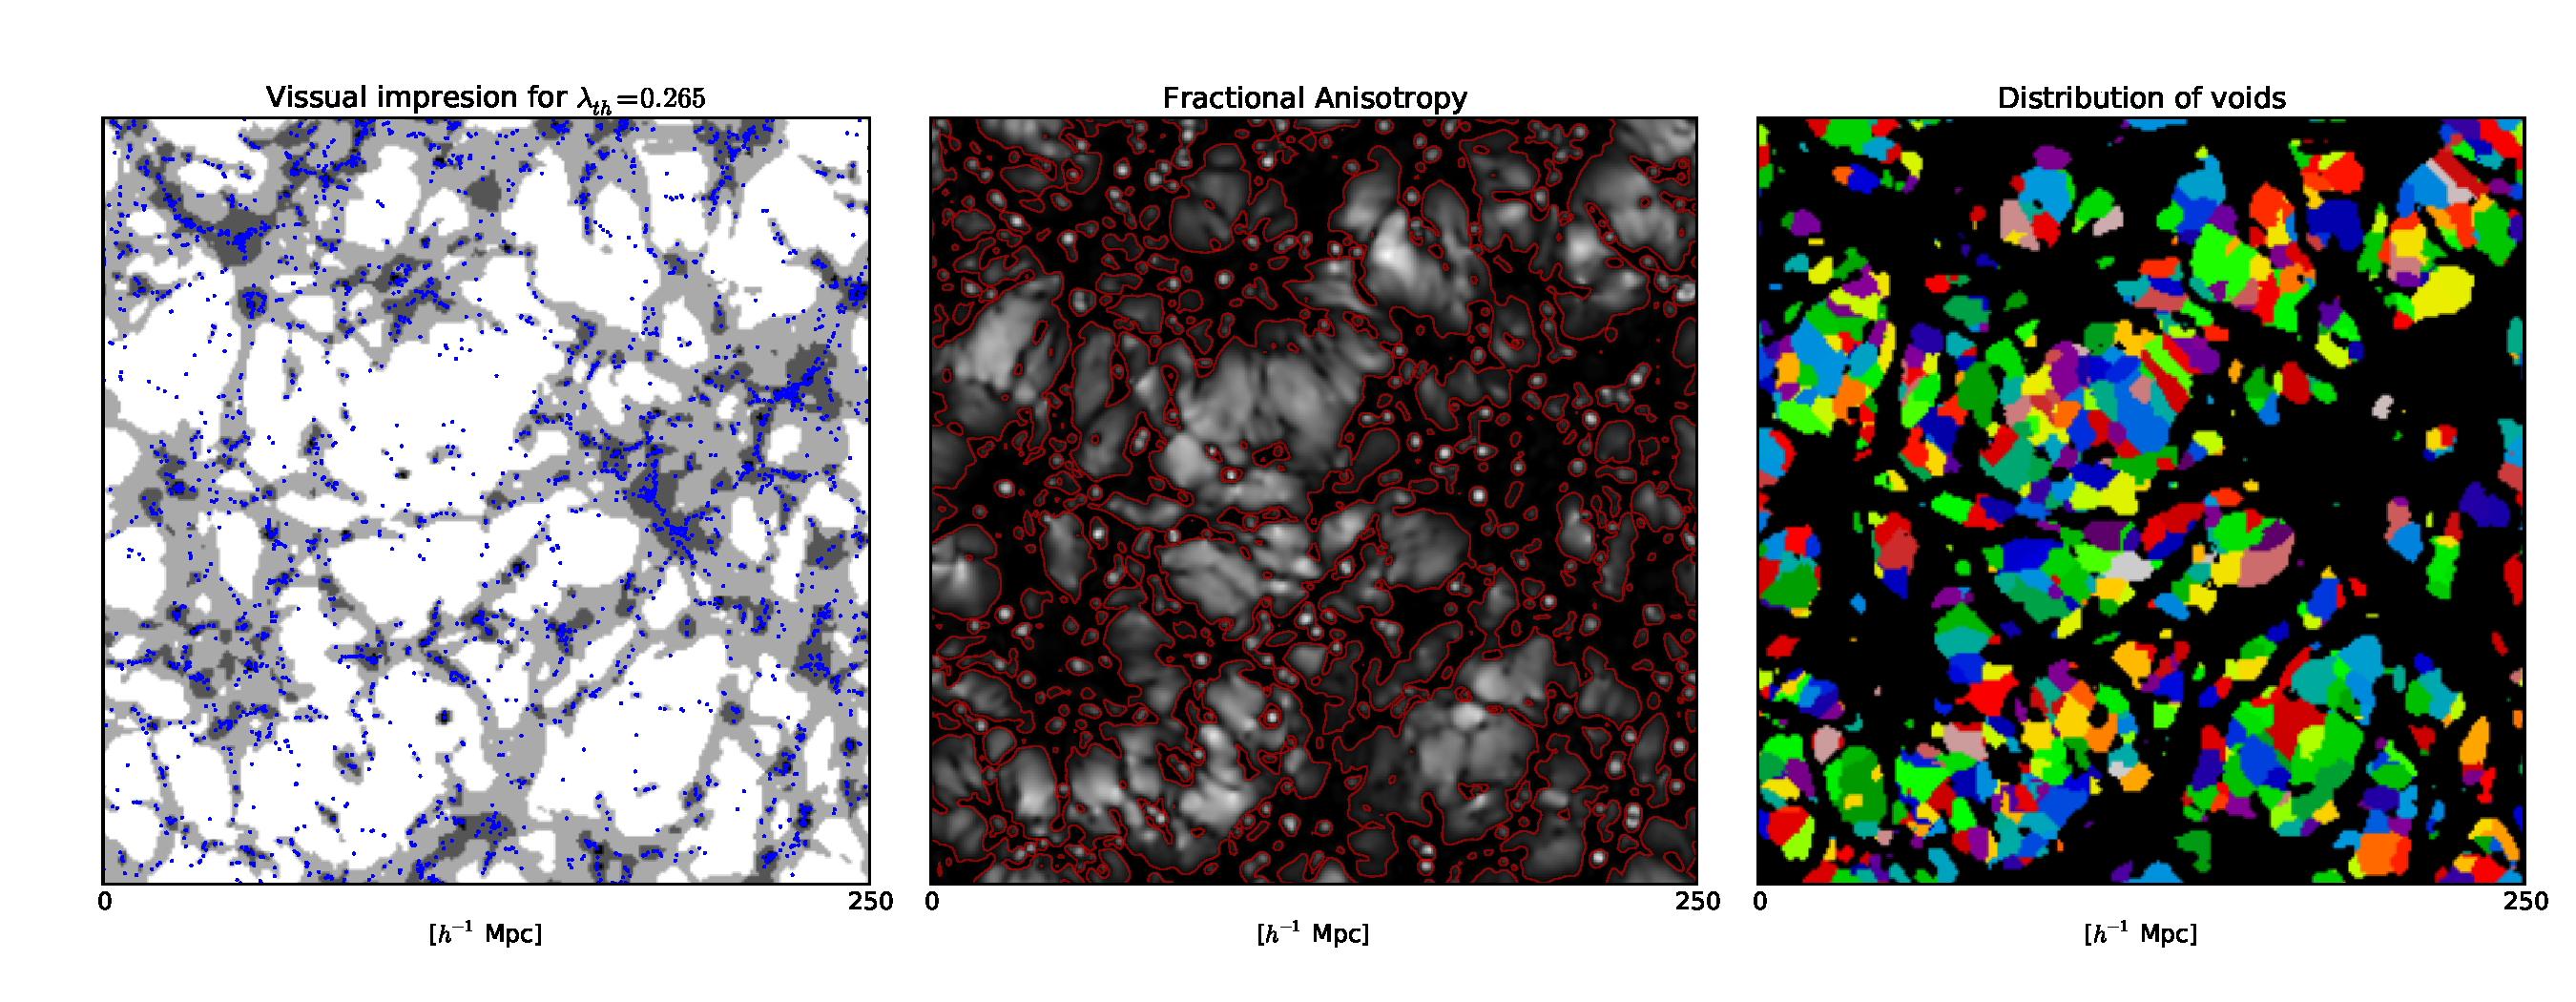
\includegraphics[trim = 16mm 10mm 5mm 12mm, clip, keepaspectratio=true,
  width=0.73\textheight]{./figures/cosmicweb_FA_Tweb.pdf}
  \vspace{0.1 cm}
  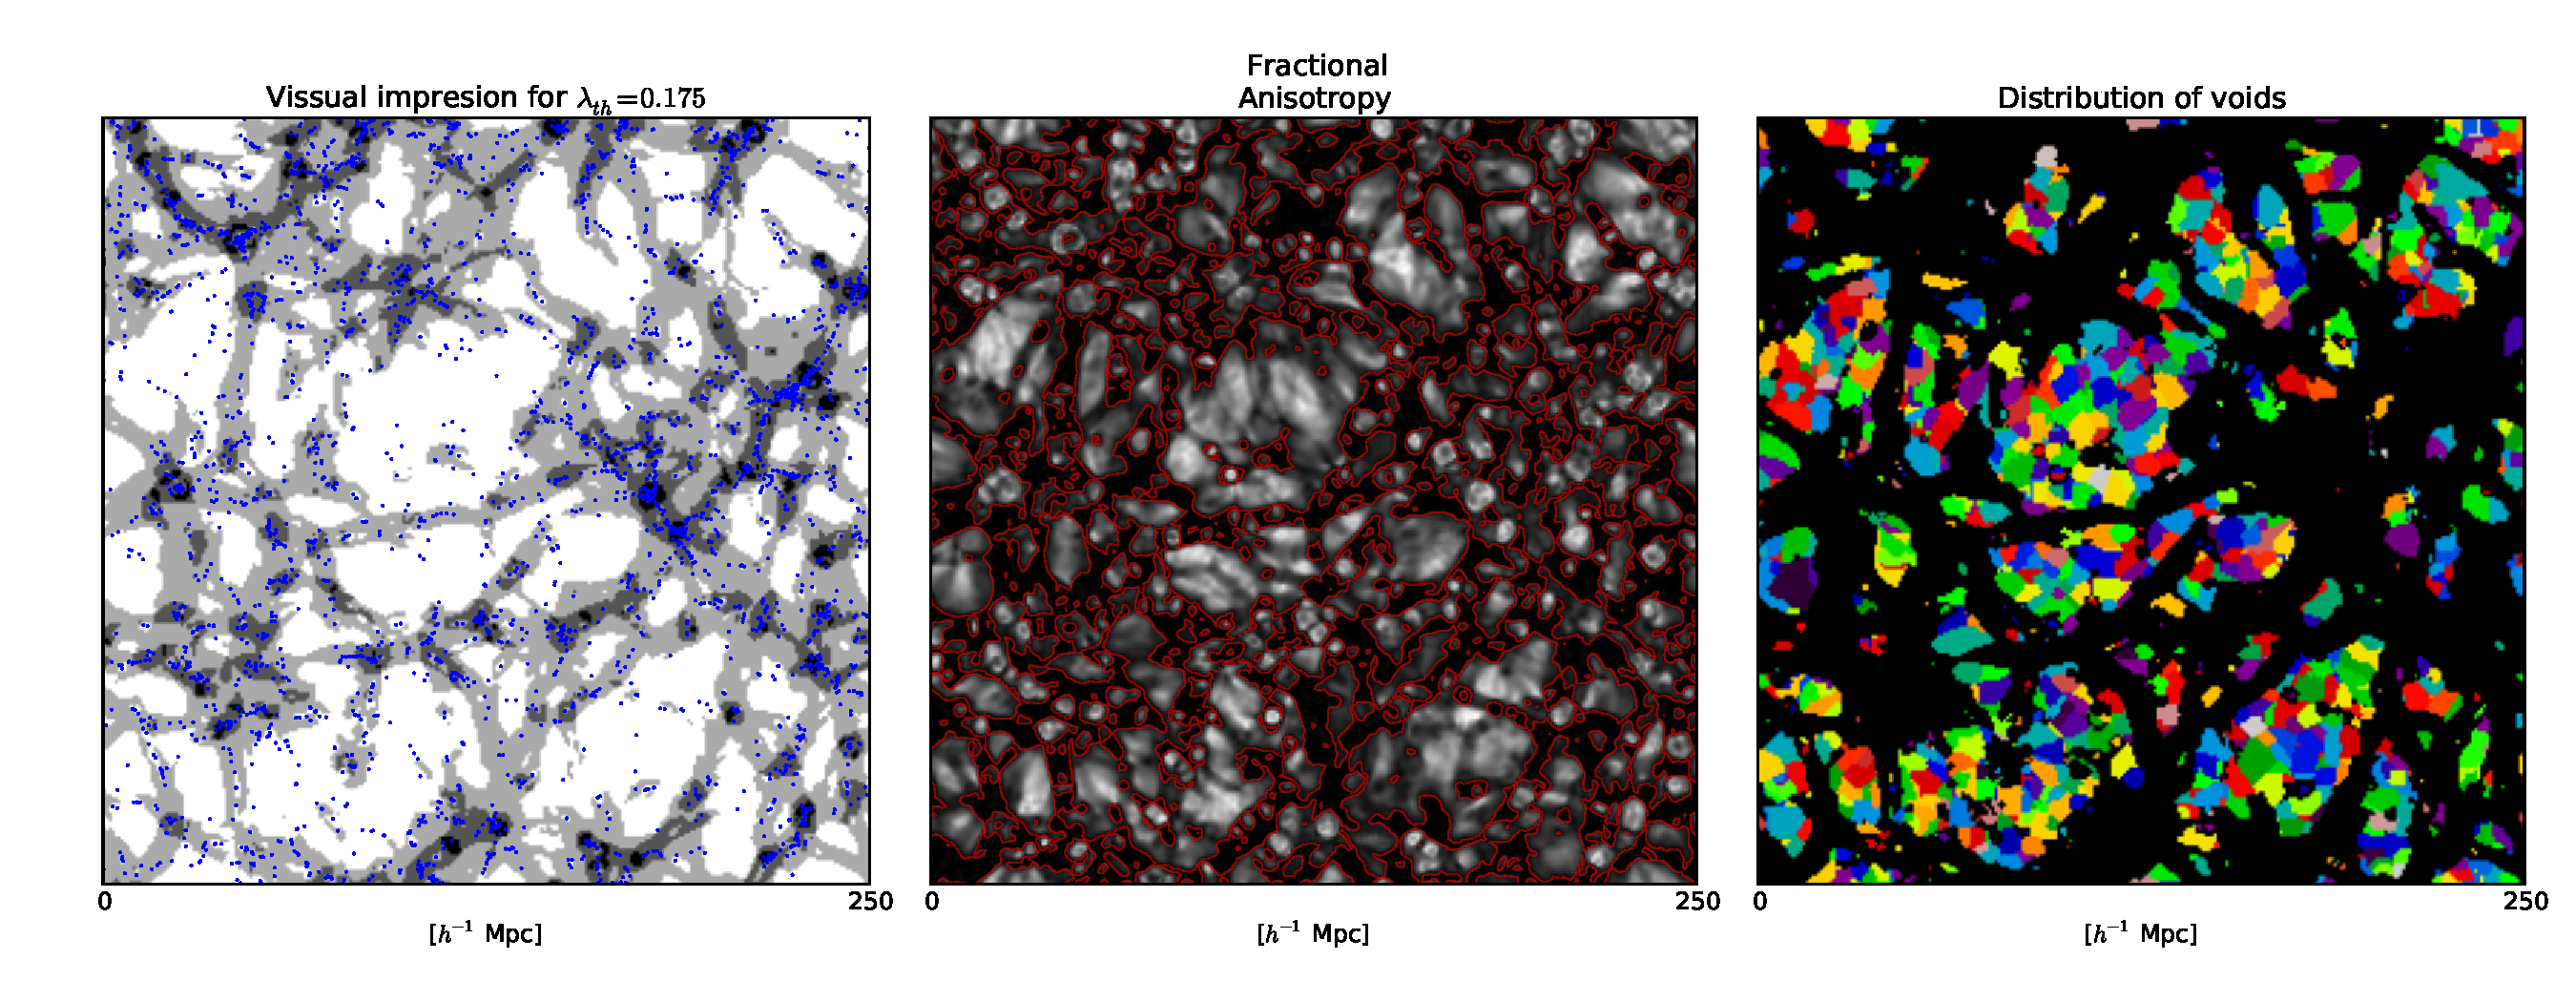
\includegraphics[trim = 16mm 10mm 5mm 12mm, clip, keepaspectratio=true,
  width=0.73\textheight]{./figures/cosmicweb_FA_Vweb.pdf}
  
  \captionof{figure}{\small Left panels show the visual impression of the 
  FA field over a slide of the simulation for each web scheme (T-web, upper 
  panels. V-web, middle panels). Black regions correspond with high values, 
  i.e. FA$\approx 1$, while white and light yellow regions to FA$\approx 0$. 
  It is worth noting the degeneration of low values of FA for knots and 
  central regions of voids, thus indicating a high isotropy for both 
  processes. In the same way, high values of FA are consistent with the 
  anisotropic geometry exhibited by filaments and very flat sheets. Middle 
  panels sketch the components of the Cosmic Web using the optimal threshold 
  values. Voids corresponds with white, sheets to gray, filaments to dark 
  gray and knots with black regions. Finally right panels sketch the 
  distribution of the catalogued voids by our method.}

  \label{fig:FA_field}

  
\end{figure*}
%.........................................................................


%.........................................................................
%FIGURE 2: Distributions of FA and density regarding the Lambda_1 eigenvalue
\begin{flushleft}
\begin{figure*}
\centering

  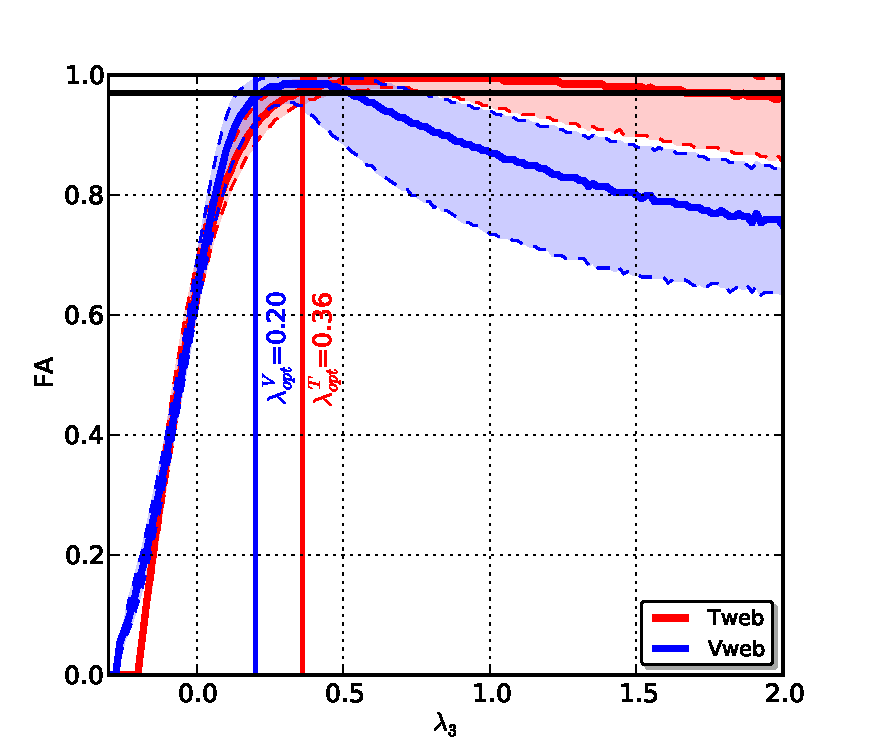
\includegraphics[trim = 2mm 2mm 5mm 10mm, clip, keepaspectratio=true,
  width=0.3\textheight]{./figures/FA_L1.pdf}
  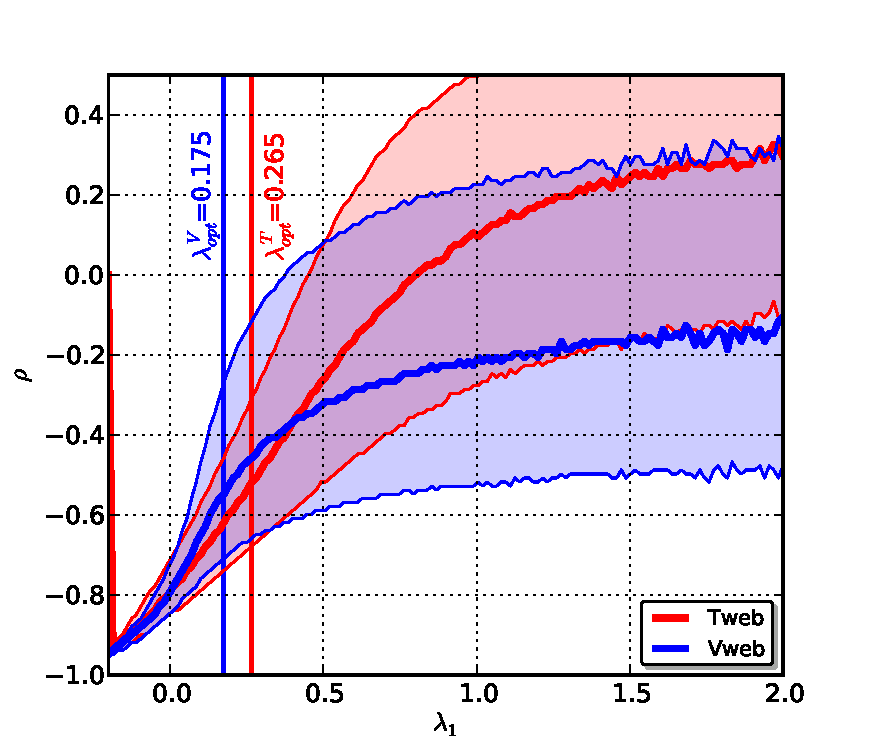
\includegraphics[trim = 2mm 2mm 5mm 10mm, clip, keepaspectratio=true,
  width=0.3\textheight]{./figures/delta_L1.pdf}  
  
  \captionof{figure}{\small Distributions of the FA (left panel) and the 
  density field (right panel) with respect to the eigenvalue $\lambda_1$ 
  for each web scheme (Tweb, red lines. Vweb, blue lines) as calculated 
  over all cells of the grid. Thick central lines correspond with the median 
  and filled regions with the $50\%$ of the distribution.}

  \label{fig:L1_correlations}
  \vspace{0.1 cm}

\end{figure*}
\end{flushleft}
%.........................................................................


%.........................................................................
%FIGURE 3: FA of some regions and shape illustration
\begin{flushleft}
\begin{figure*}
\centering

  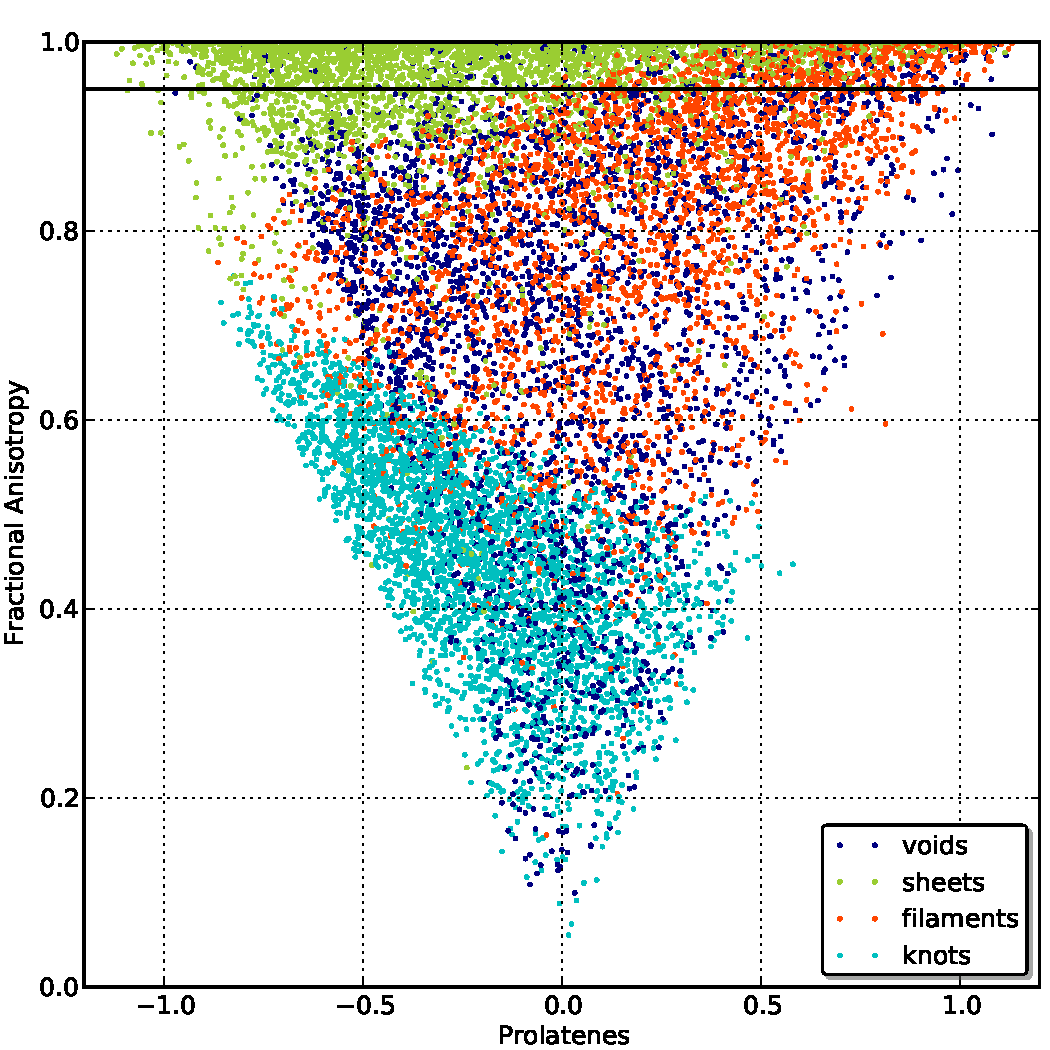
\includegraphics[trim = 0mm 1mm 0mm 1mm, clip, keepaspectratio=true,
  width=0.3\textheight]{./figures/FA_Prolatenes_Vweb.pdf}
  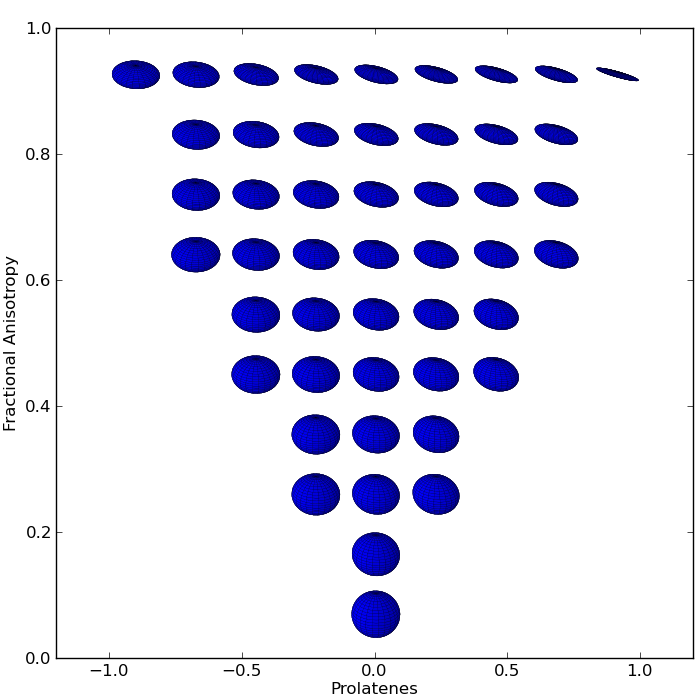
\includegraphics[trim = 0mm 1mm 0mm 1mm, clip, keepaspectratio=true,
  width=0.3\textheight]{./figures/FA_Prolatenes.png}  
  
  \captionof{figure}{\small Fractional anisotropy and prolateness for a 
  random sample of cells (left panel) and for different spherical 
  geometries (right panel). For the cells, each environment is coded with
  a different colour, i.e. voids corresponds with dark blue points, 
  sheets with green, filaments with orange and knots with cyan. The axis 
  of the spheroids are computed from the relative strengths of the 
  eigenvalues, so their shape sketch the relative expanding/collapsing 
  dynamics into each direction.}

  \label{fig:FAShapeness}
  \vspace{0.1 cm}

\end{figure*}
\end{flushleft}
%.........................................................................


%.........................................................................
%FIGURE 4: volume functions
\begin{flushleft}
\begin{figure*}
\centering

  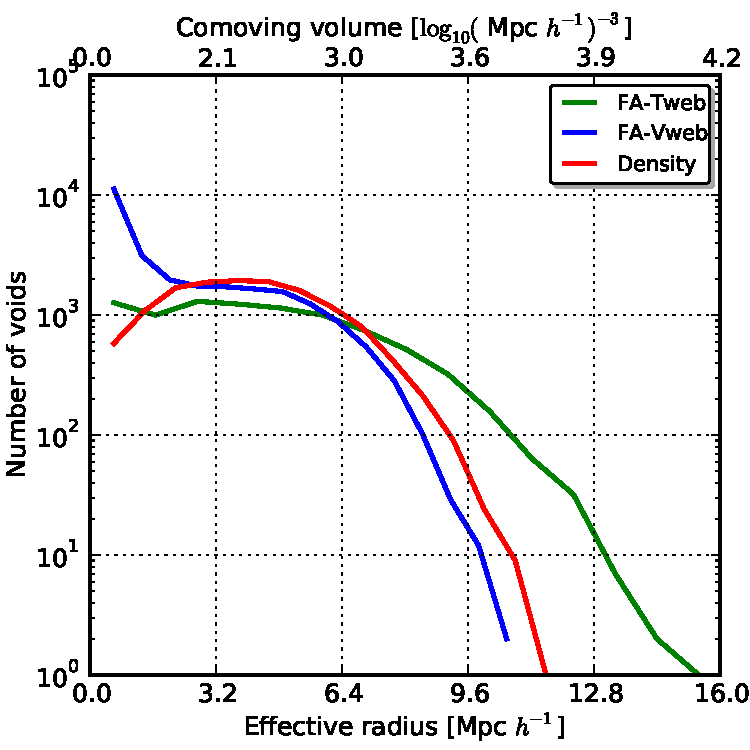
\includegraphics[trim = 0mm 0mm 0mm 0mm, clip, keepaspectratio=true,
  width=0.3\textheight]{./figures/voids_regions_volume_all.pdf}
  
  \captionof{figure}{\small Volume functions of voids for both built 
  catalogues. Watershed-Tweb (red curves), Watershed-Vweb (blue curves).
  Continuous lines corresponds with the total number of voids, dot-dashed
  with sub-compensated voids and dashed lines with over-compensated voids. }

  \label{fig:volume_function}
  \vspace{0.1 cm}

\end{figure*}
\end{flushleft}
%.........................................................................


%.........................................................................
%FIGURE 5: Density profile of voids for each defined scheme
\begin{flushleft}
\begin{figure*}
\centering
  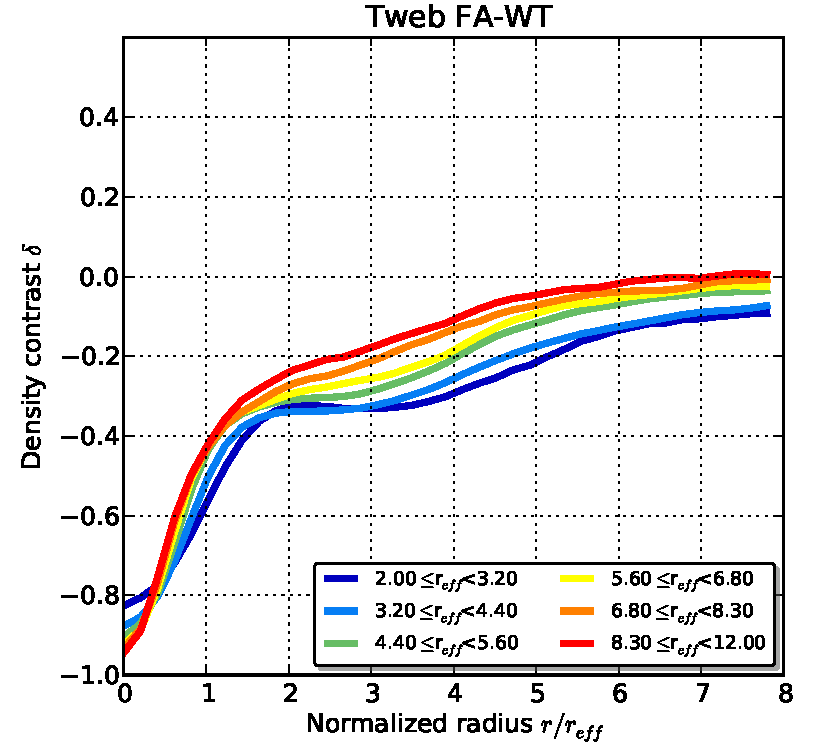
\includegraphics[trim = 1mm 0mm 5mm 0mm, clip, keepaspectratio=true,
  width=0.24\textheight]{./figures/voids_density_TwebFAG0.pdf}
  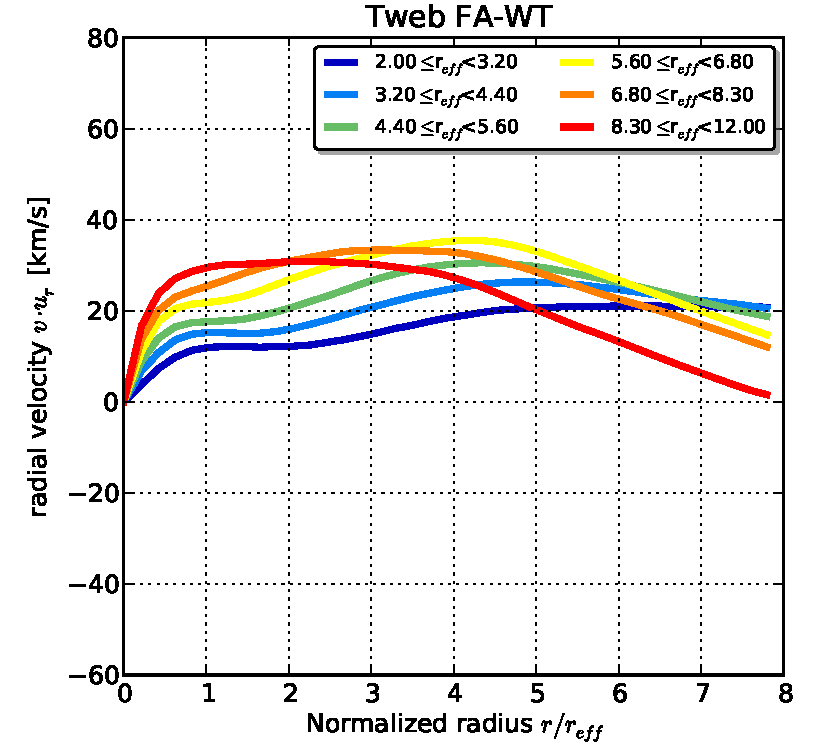
\includegraphics[trim = 1mm 0mm 5mm 0mm, clip, keepaspectratio=true,
  width=0.24\textheight]{./figures/voids_velocity_TwebFAG0.pdf}
  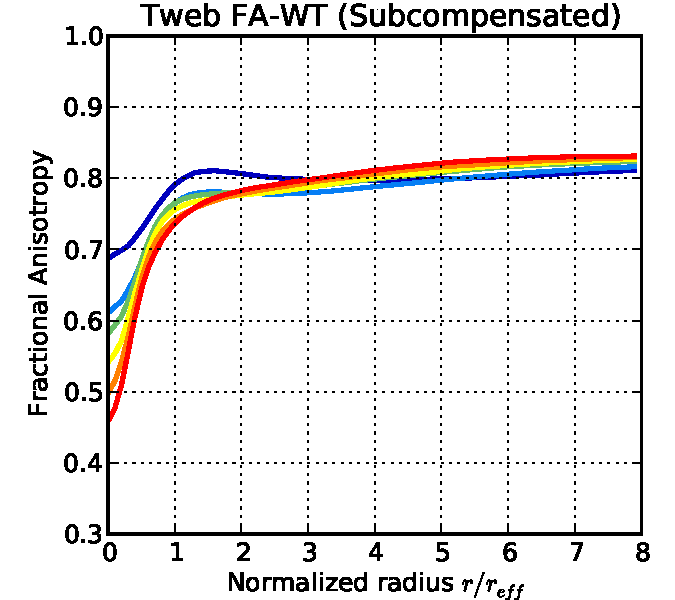
\includegraphics[trim = 1mm 0mm 5mm 0mm, clip, keepaspectratio=true,
  width=0.24\textheight]{./figures/voids_FA_TwebFAG0.pdf}
  
  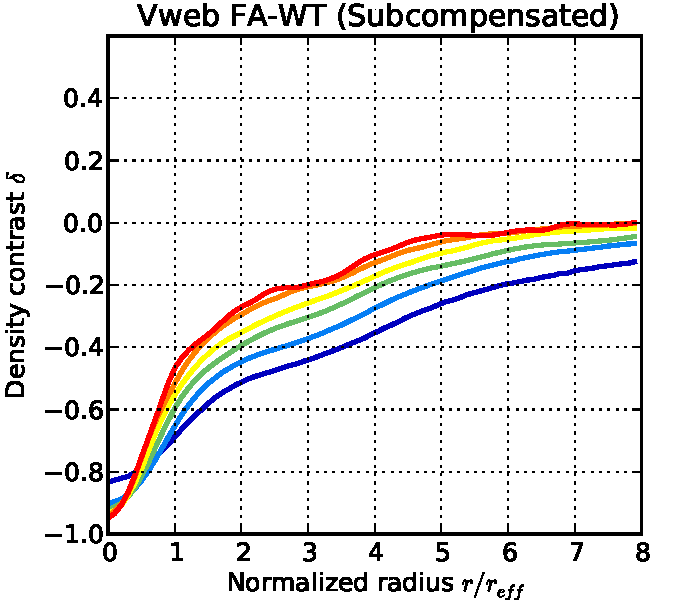
\includegraphics[trim = 1mm 0mm 5mm 0mm, clip, keepaspectratio=true,
  width=0.24\textheight]{./figures/voids_density_VwebFAG0.pdf}
  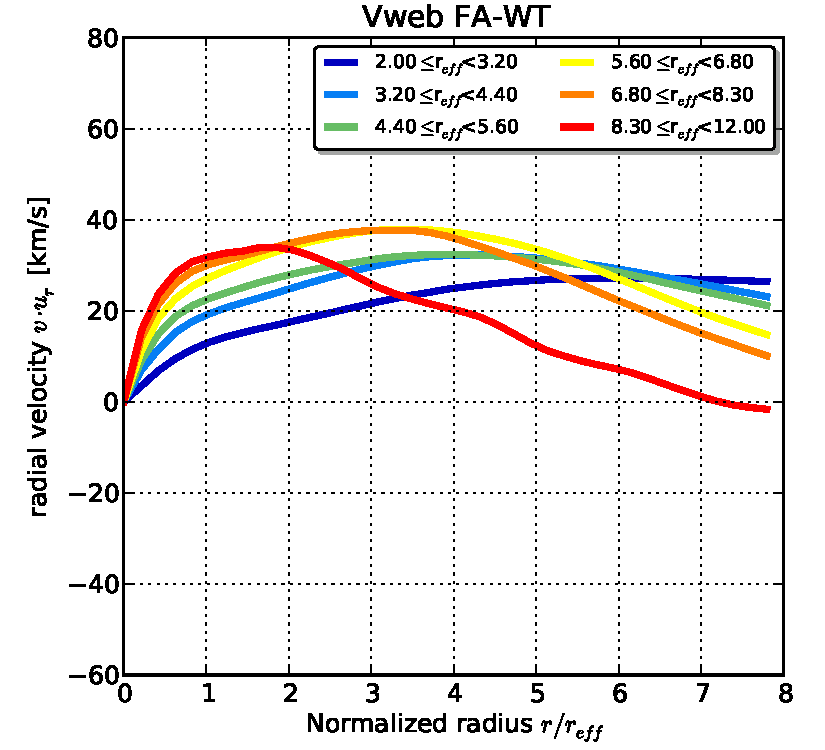
\includegraphics[trim = 1mm 0mm 5mm 0mm, clip, keepaspectratio=true,
  width=0.24\textheight]{./figures/voids_velocity_VwebFAG0.pdf}
  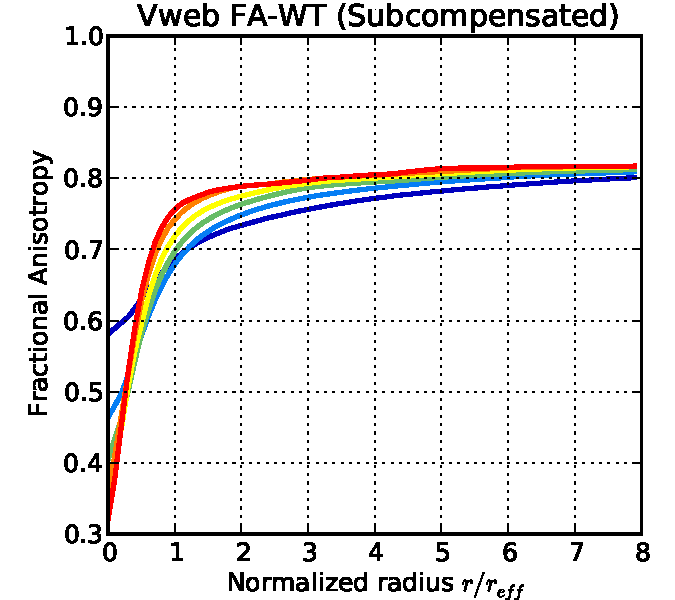
\includegraphics[trim = 1mm 0mm 5mm 0mm, clip, keepaspectratio=true,
  width=0.24\textheight]{./figures/voids_FA_VwebFAG0.pdf}
  
  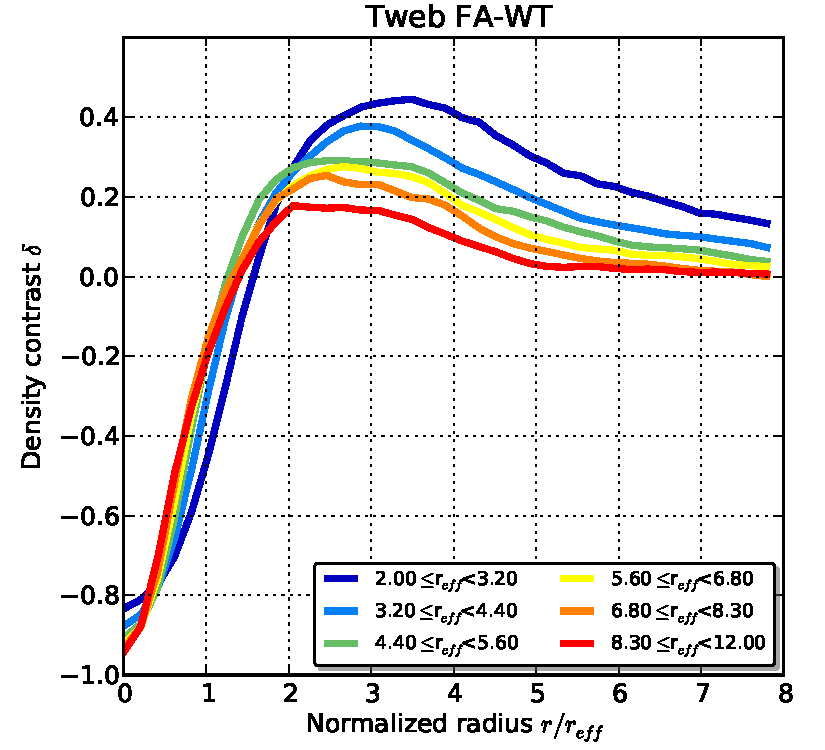
\includegraphics[trim = 1mm 0mm 5mm 0mm, clip, keepaspectratio=true,
  width=0.24\textheight]{./figures/voids_density_TwebFAG1.pdf}
  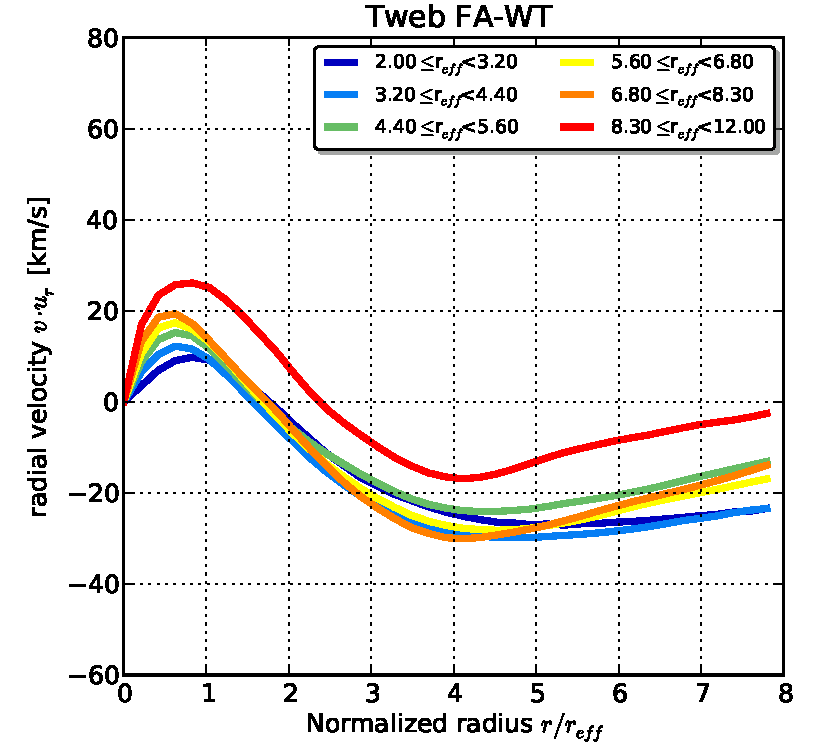
\includegraphics[trim = 1mm 0mm 5mm 0mm, clip, keepaspectratio=true,
  width=0.24\textheight]{./figures/voids_velocity_TwebFAG1.pdf}
  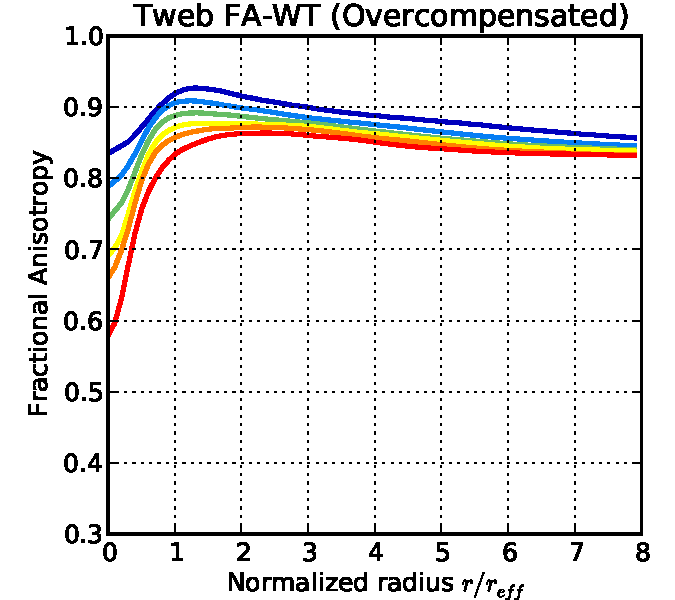
\includegraphics[trim = 1mm 0mm 5mm 0mm, clip, keepaspectratio=true,
  width=0.24\textheight]{./figures/voids_FA_TwebFAG1.pdf}

  
  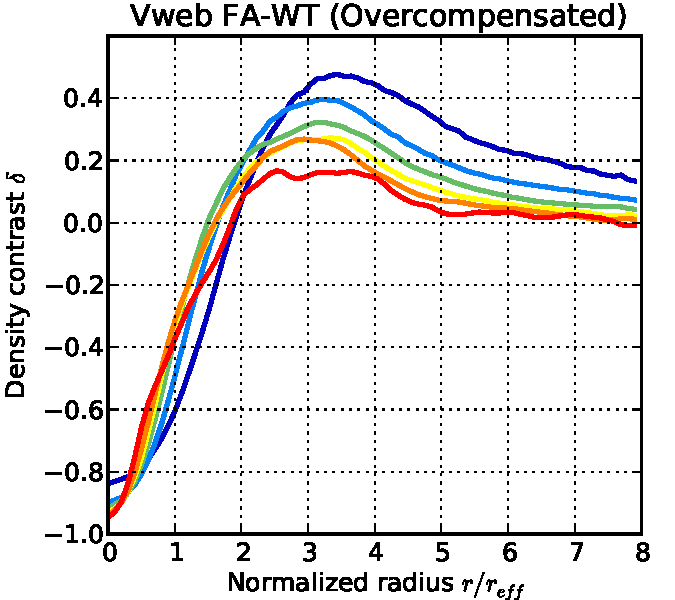
\includegraphics[trim = 1mm 0mm 5mm 0mm, clip, keepaspectratio=true,
  width=0.24\textheight]{./figures/voids_density_VwebFAG1.pdf}
  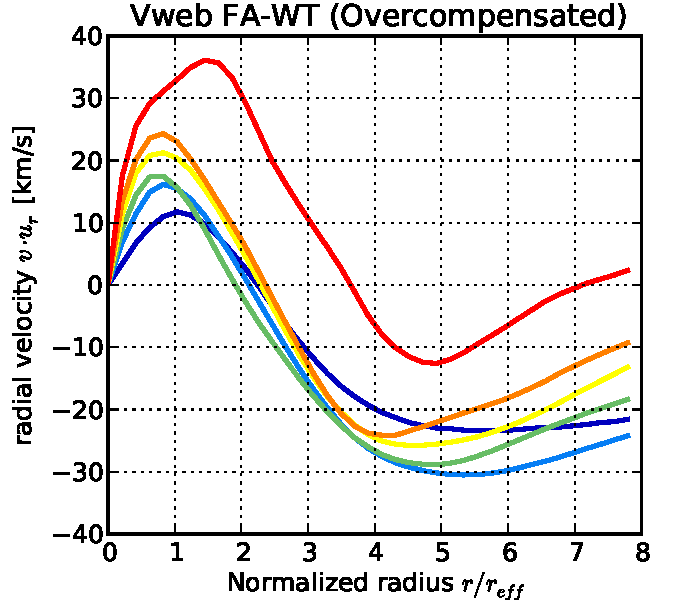
\includegraphics[trim = 1mm 0mm 5mm 0mm, clip, keepaspectratio=true,
  width=0.24\textheight]{./figures/voids_velocity_VwebFAG1.pdf}
  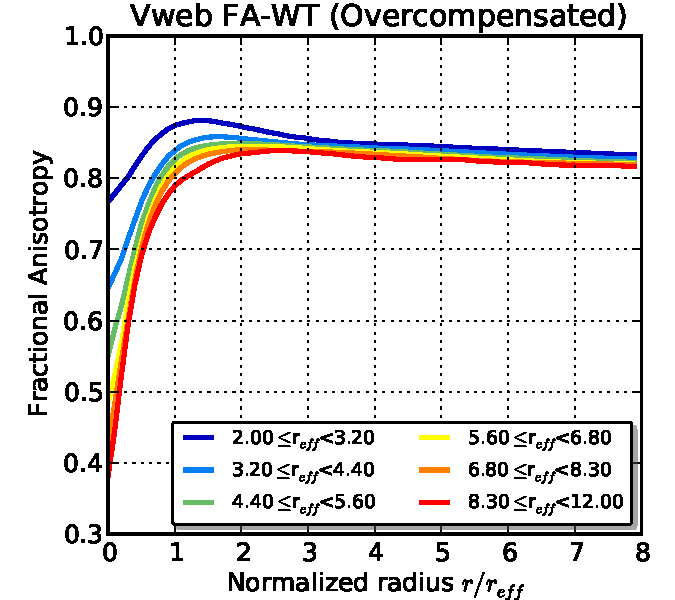
\includegraphics[trim = 1mm 0mm 5mm 0mm, clip, keepaspectratio=true,
  width=0.24\textheight]{./figures/voids_FA_VwebFAG1.pdf}  
  

  \captionof{figure}{\small Density of voids for each finding scheme.}

  \label{fig:RhoVel}
  \vspace{0.1 cm}

\end{figure*}
\end{flushleft}
%.........................................................................


\end{document}
